%!TEX root = ../USthesis_Masters.tex
\chapter{Detail Design}
\label{chp:Detail Design}


%%%%%%%%%%%%%%%%%%%%%%%%%%%%%%%%%%%%%%%%%%%%%%%%%%%%%%%%%%%%%%%%%%%%%%%
\section{Back-end}

To implement the payment framework, we need a back-end server and a back-end web framework. 

\subsection{Back-end Server}

We chose an Amazon Elastic Cloud Computing (EC2) instance for the back-end server. EC2 gives us access to a virtual machine (VM) where we can run our own software, including a publicly accessible website. The micro instance is deployed in Singapore in the Asia Pacific region. The reason for this is to have the server as close as possible to the WeChat servers in China, since our servers must connect to WeChat's servers.

\subsection{Back-end Web Framework}
\label{sct:web_framework}
We decided to use XAMPP (Apache, MySQL, PHP and Perl) for the back-end development environment. XAMPP is a full stack development environment. It includes an HTTP server (Apache), a database server (MySQL) and a scripting language (PHP). XAMPP is free and easy to deploy, and is also used because the author is familiar with it.

\section{Social Media Platform}

We chose WeChat for our social media platform. WeChat works on most smartphones, already has a userbase and it has a third-party API with a development sandbox feature. 

On WeChat, a third-party application is known as an ``Official Account''. We registered for a sandbox Official Account that only allows 20 users and is not searchable on WeChat.

WeChat acts as an intermediary between the user and our server as seen in figure \ref{fig:wechat_interaction}. 

\begin{figure}
  \centering
    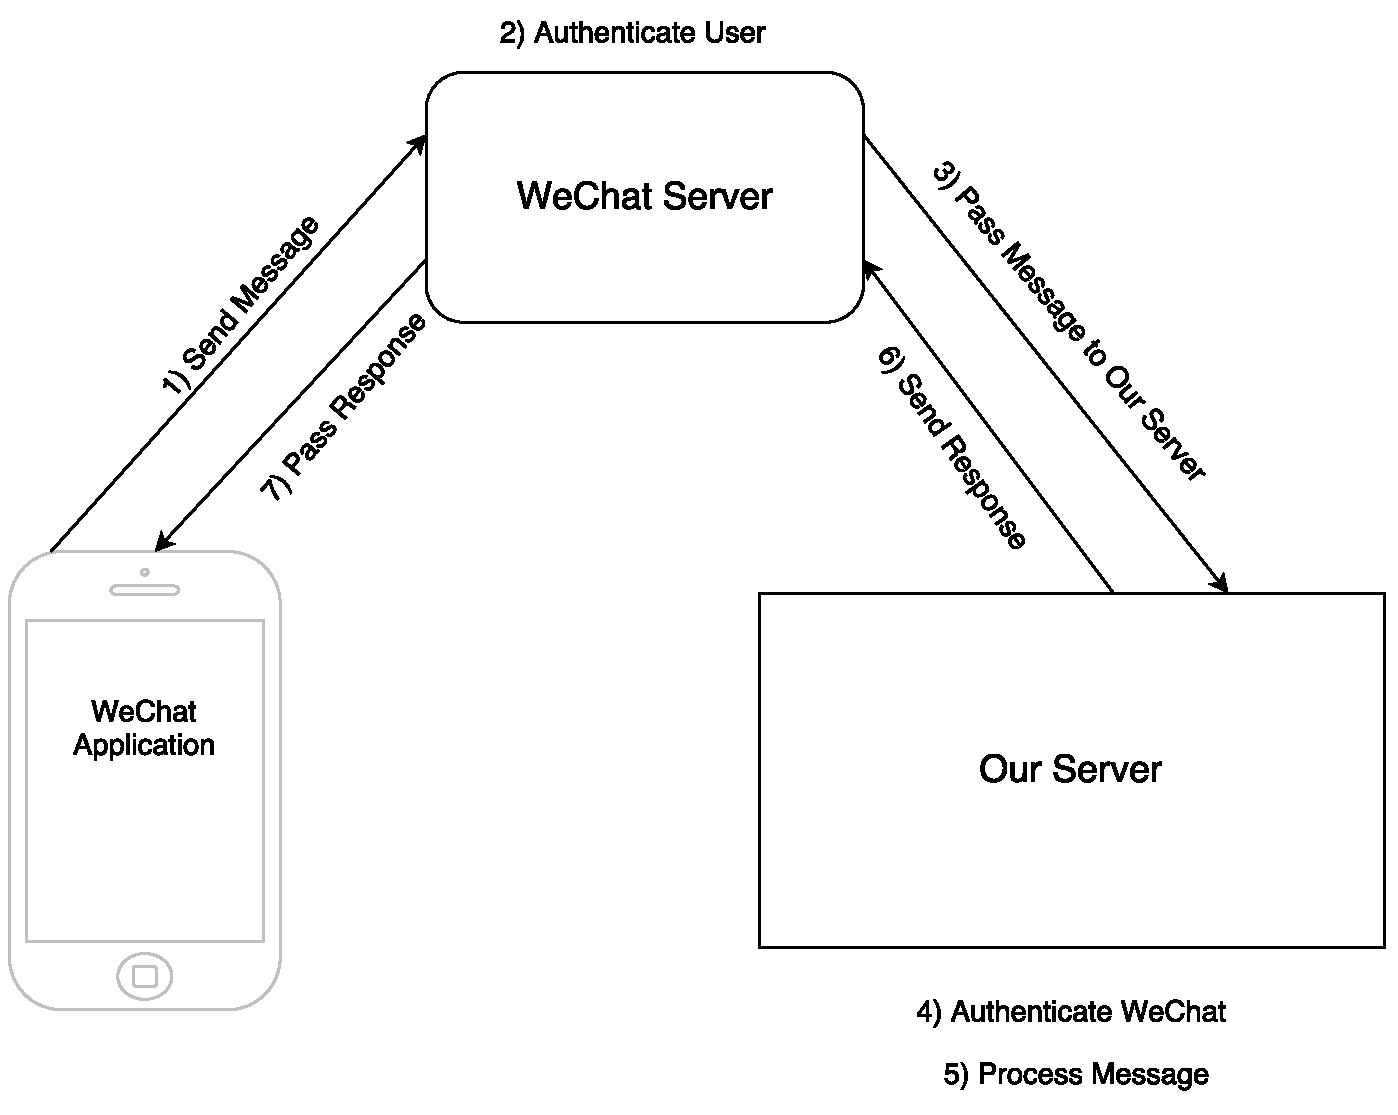
\includegraphics[width=0.7\textwidth]{figs/Wechat_interaction.pdf}
   \caption{Interaction with WeChat} 
   \label{fig:wechat_interaction}
\end{figure}

\subsection{WeChat Security}
\label{sct:wechat_security}

WeChat uses a shared token hashing scheme to authenticate itself on our server. We provide WeChat with a unique string to use for authentication purposes. That string is then used in every request that is made to our server. WeChat uses the string we provided, a random nonce and the UNIX timestamp to create a signature. It sorts the string, timestamp and nonce and forms a single string from these three values. This single string is then hashed using the SHA256 hashing algorithm to generate a signature. When a request is made to our server, WeChat provides the nonce, the timestamp and the signature The message does not contain the unique string. Since we know the unique string, we can use the nonce and timestamp to also generate a signature. If the message comes from someone that possesses the same unique string, the signature that is provided must match the signature that we calculated.

Thus, we can be reasonably certain that any request that is made to our server with a signature that is verified comes from WeChat and not an attacker. If our unique string is compromised somehow, someone will be able to make false requests to our server that appear valid. If this would happen, we can give WeChat a new unique string. 

\subsection{WeChat Interface}

The WeChat Official Account interface works on a message-answer basis. Any message that the user sends in the Official Account dialog is forwarded to our server. When we configure our Official Account, we provide WeChat with a URL that points to the script that handles all messages from and to Wechat. This script verifies any incoming messages as described in section \ref{sct:wechat_security}.

The incoming message is in XML format. It contains a unique identifier for every subscriber to the WeChat Official Account. It is important to note that the unique identifier is only unique for the spesific Official Account. The identifier is not a global unique identifier for the entire WeChat platform. Thus, the same user will have two different identifiers in two different Official Accounts. This is important to remember, since we will be using two seperate Official Accounts.

The messages that are received must be interpreted and responded to accordingly. Since we will have applications that rely on previous messages and results, we need something to keep track of the user's current state. A state machine is required to look at the current state the user is in, look at the message they sent and accordingly determine what to reply and to what state to move to. 

To keep track of the user's state, we will use a MySQL database as described in section \ref{sct:web_framework}. Thus, for each message received, we will read the user's current state from the database and apply the state machine logic to their message. We will then update their state in the database and reply with the message that the state machine determined.

\subsection{Gamebook Design}
\label{sct:gamebook_design}

The use-case application we chose to demonstrate the payments framework is a Gamebook application. A Gamebook is a non-linear book that tells a story based on the user's input. In physical books, this is done by giving the user a choice and then telling them what page to go to based on their choice. In the digital realm, we can simply provide the user a choice and give them the corresponding text. The software keeps track of what options links where.

In a dedicated Gamebook reader, a common method of generating a Gamebook is using a scripting language like ChoiceScript \cite{LLC}. Since WeChat doesn't have any client-side scripting, using a scripting language like this is not possible. 

We decided to create our own system of storing and reading Gamebooks. We use the MySQL database as the method of storing and organising the Gamebooks.

\subsubsection{Gamebook Database Design}

Every book in our design is a table, and every page is an entry in the table. Each entry has a unique id, the text of the page and then the references of each of the choices from that page. We chose five to be the maximum amount of choices on each page. The database resembles a linked list, where each entry has pointers to the next corresponding entry. The design of the Gamebook table is seen in figure \ref{fig:gamebook_database}.

\begin{figure}
  \centering
    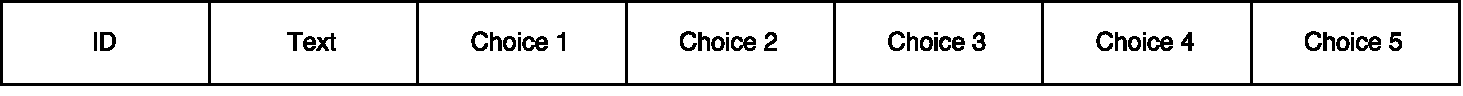
\includegraphics[width=0.7\textwidth]{figs/Gamebook_Database.pdf}
   \caption{Gamebook Database Table} 
   \label{fig:gamebook_database}
\end{figure}

The values of the fields choice 1 - 5 will have the corresponding ID's of the ``page'' they link to. If an entry only has two choices, the rest of the options will have the value null to indicate that it is not a valid choice.

We chose this method of storing the Gamebooks, because it is easy to implement, easy for a writer to visualise and allows us to have sircular stories and also allows us to visit multiple branches of the story. 

We will also need two more tables: one to store a list of all the books available and another to keep track of books purchased by individuals. 

\subsubsection{Gamebook Author Platform}

As stated in section \ref{sct:gamebook_design}, we are not going to use a scripting language to write the Gamebook in. It doesn't fit the design of the application that we are building, and has a learning curve for people that want to start writing books and are not familiar with scripting languages. We decided to use a Graphical User Interface for writing the Gamebooks.

We decided to use a website as the author platform. We used commonly used web technologies to build the platform. For the front-end, we used HTML, JavaScript with jQuery, and Twitter's Bootstrap CSS framework.

Using AJAX, we connect the front-end with the back-end PHP scripts that connects to the MySQL database. We also decided to use an OAuth login mechanism to facilitate logins, rather than writing our own login system. A big motivation for doing this is the authors desire to get experience with OAuth. We decided to use Google's OAuth platform, because it widely used and well documented. By using OAuth, we are enabled to have unique, secure logins without having to design all the security measures to protect the user. It also makes it easier for the user, because they can log in with a single click.

Since the Gamebook resembles a tree, we decided to display the tree using an organisational chart. We used Google's JavaScript Chart API to map the Gamebook. The Chart API is free, simple, powerful and well documented. To display the story as a tree makes it easier for the writer to navigate through the book and to get a bigger picture of the story. An example of such a chart can be seen if figure \ref{fig:gamebook_tree}. Using a chart makes it easier for the author to see where the story needs more work.

\begin{figure}
  \centering
    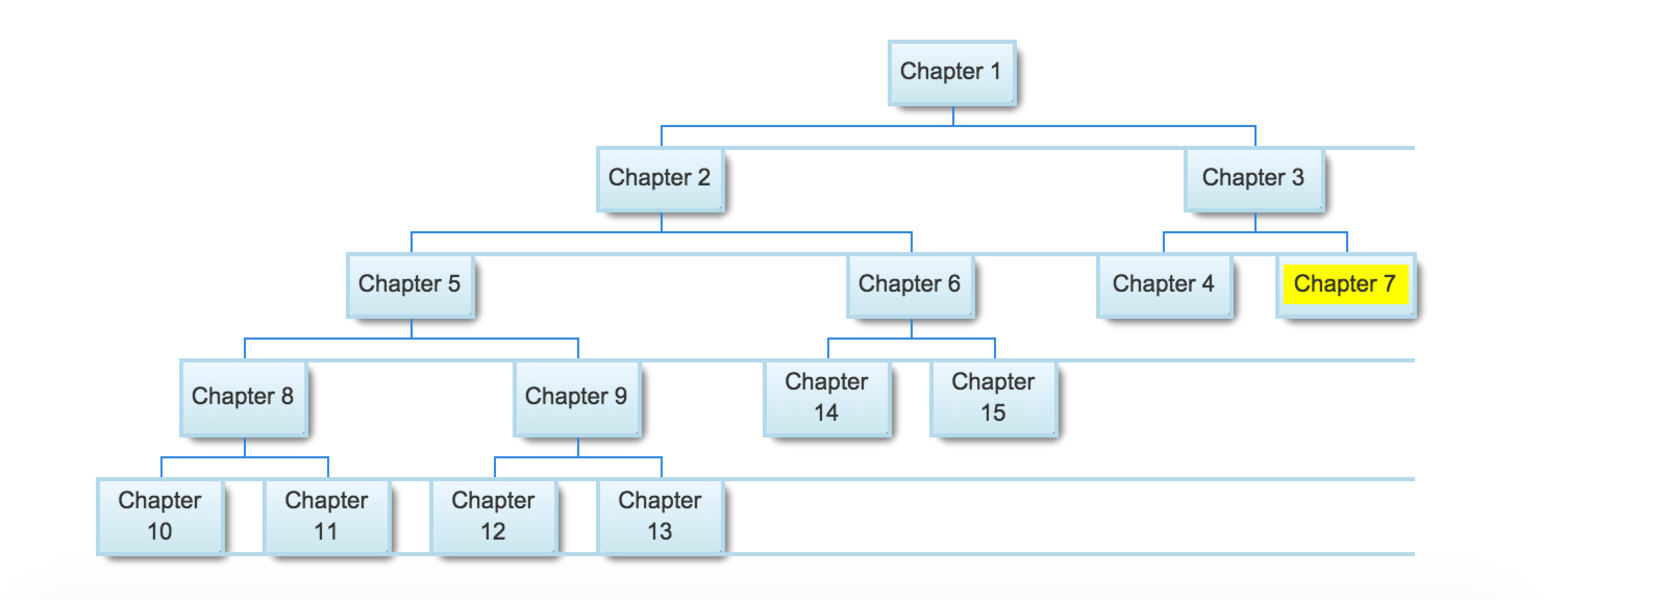
\includegraphics[width=\textwidth]{figs/gamebook_tree.pdf}
   \caption{Gamebook Tree Representation} 
   \label{fig:gamebook_tree}
\end{figure}


\section{WeChat Wallet Design}
\label{sct:wechat_wallet_design}

As stated before, the WeChat Official Account doesn't allow us to run client-side code. This means that the WeChat Wallet will have to be a hosted Bitcoin wallet, with the Official Account interfacing with the hosted wallet.

To have a WeChat wallet, we need a Bitcoin address. When hosting a Bitcoin wallet, there are two main method of keeping addresses. The first method is where a user gets a single address or adresses and these addresses are used only by the single user. The user may or may not have access to the private key, but the wallet is associated with only that user. This allows the user to verify the balance and transactions by checking the blockchain. 

The second method is where the user has an account, and can have a receiving address, but the user is not directly in control of the address. The users' balance is not verifiable by using the Bitcoin blockchain. This is because the server keeps track of the balance of the user, and makes a payment from other addresses when a user wants to make a payment.

We chose the first method of storing the address, because it is simpler and has a more direct feeling for the user that he is using a real Bitcoin wallet, and not just something that arbitrarily keeps track of the balance.

\subsection{Bitcoin Interface Design}
\label{sct:bitcoin_interface_design}

Thus, we need to generate a Bitcoin address for each user. To do this, we use a a popular open-source PHP Bitcoin library called bitcoin-lib-php. One of the features of Bitcoin is that generating a Bitcoin wallet can be done locally. That means that the bitcoin-lib-php library generates a Bitcoin address on our server without connecting to the Bitcoin network. This has many advantages, including it doesn't use network bandwidth, it is fast and the private key never leaves our server.

We chose bitcoin-lib-php as our library, because it satisfies our requirements perfectly, it is open-source (and thus verifiable) and is decently documented. 

As mentioned in section \ref{sct:wechat_wallet_design}, by creating an address for each user, the user can more directly monitor his funds and transactions since it can be independently verified by using any software that is connected to the Bitcoin blockchain.

The Bitcoin library allows us to create an address, create a Bitcoin transaction and sign a transaction. These are the core functions of Bitcoin. However, a transaction can't be created without information about the address or addresses that want to create the transaction. This information is called ``unspent outputs'' and, as the name suggests, are previously received transactions that are not yet spent. These unspent outputs contain all the information to build a transaction, including the value of the output, the transaction hash and the script type etc.

These unspent outputs are only acquirable with access to the Blockchain and we do not run the Bitcoin software. Thus we do not have direct access to these outputs. From our requirements in section \ref{sct:bitcoin_interface}, we require a third-party Bitcoin interface to provide these outputs among other things. From the requirements listed in section \ref{sct:bitcoin_interface}, we decided to use chain.com. Chain.com satisfies all our requirements and is free at the time of writing. 

During the progress of this project, chain.com has release version 2 of their API with the biggest change being that they can also sign a transaction for you. When we started, we had to sign the transaction ourselves. Signing the transaction ourselves exposes us to a smaller risk of compromising the security of the users' private key. We choose to still use version 1 of the API, because updating to version 2 will not have a significant effect on our proof of concept's overall outcome. The summary of the Bitcoin payment flow can be seen in figure \ref{fig:bitcoin_payment_flow}.

\begin{figure}
  \centering
    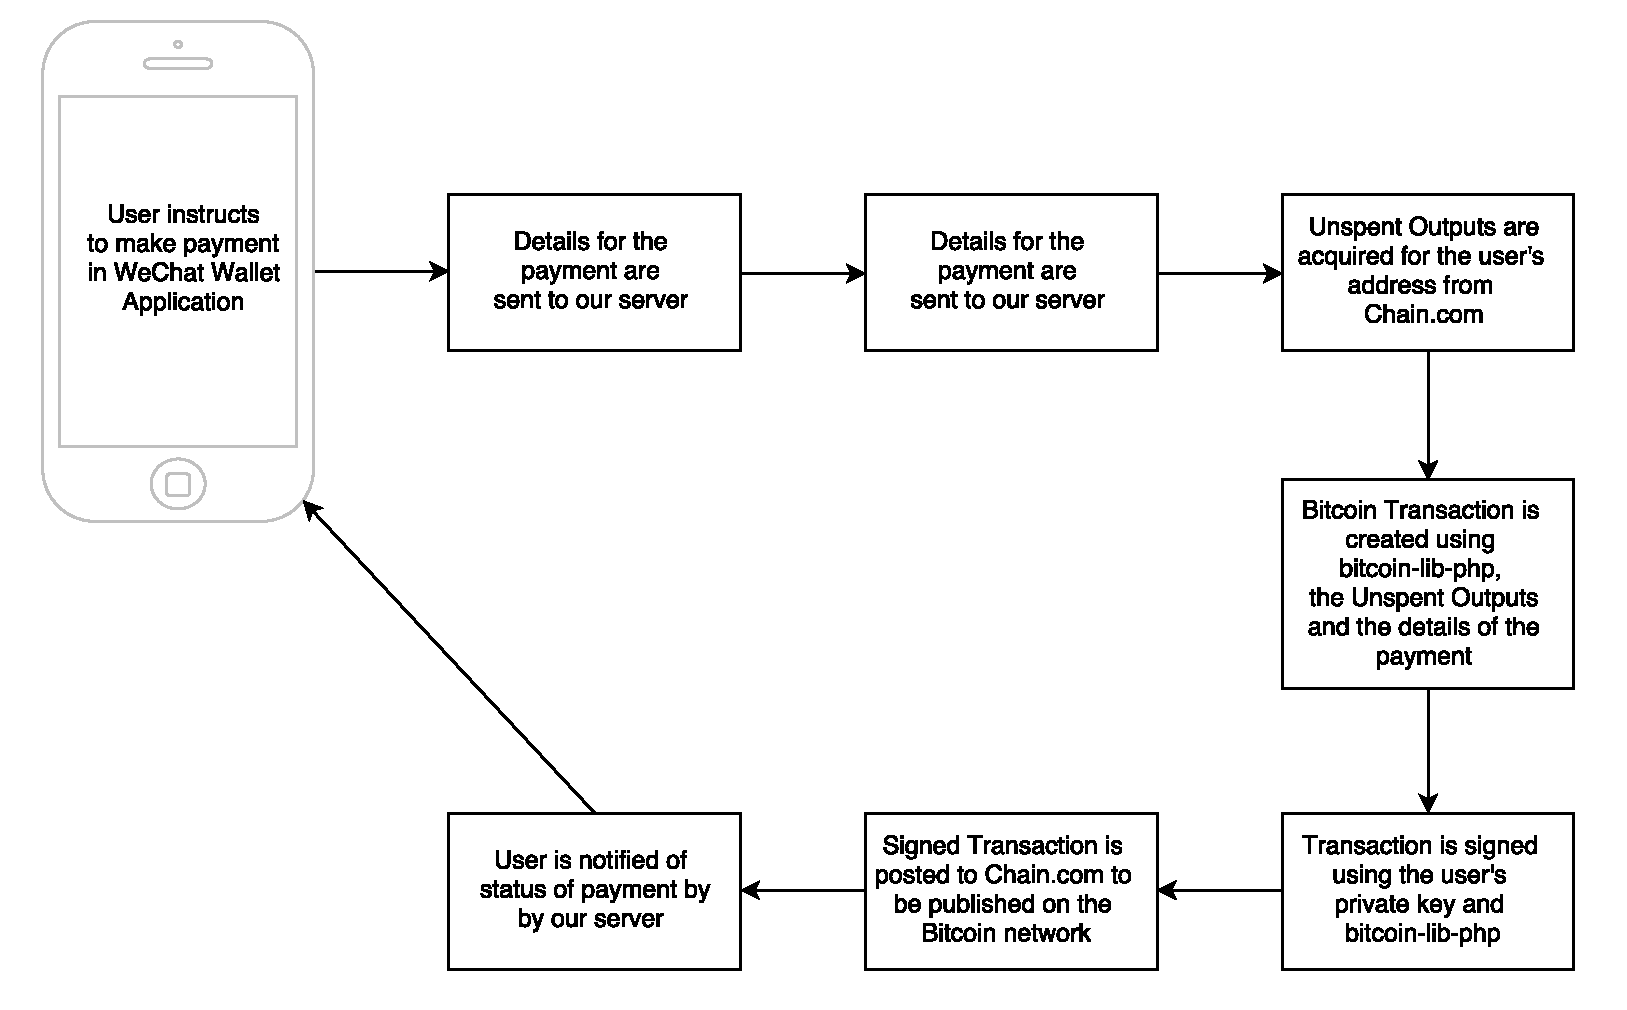
\includegraphics[width=\textwidth]{figs/Bitcoin_payment_flow.pdf}
   \caption{Bitcoin Payment Flow} 
   \label{fig:bitcoin_payment_flow}
\end{figure}

\subsection{WeChat Wallet Features Design}

The main function of a Bitcoin wallet application is to send and receive Bitcoin. A Bitcoin address is a string of 26 to 35 alphanumeric characters. Reading an address to someone is not practical due to the long length. A very common method of representing a Bitcoin address is by using a graphical QR-code. Another user can then scan a QR-code and receive the address to make the payment to.

\subsubsection{Address to QR-code}
Our first design specification is to represent the user's alphanumeric address as a QR-code image. There are several ways we can do this. The first method is to generate the QR-image on our server and send the image to the user on WeChat. The problem with this method is that our server will be responsible for generating images, and this is computationally intensive. The second method is using a webpage that generates the QR-code client-side using JavaScript. The WeChat Official Account allows us to open a link directly in WeChat. Thus, we can send the user a link of a webpage that will generate the QR-code in WeChat's built-in browser. With this method, computation is spread to the users and not a central server. 

We chose the webpage method of generating the QR-codes. We wrote our own webpage that uses an Open Source JavaScript library to generate the QR-code. We encode the address to be generated in a GET request and send the link to the user. The link will look like this: \\https://domain.com/qr?address=1Bd5wrFxHYRkk4UCFttcPNMYzqJnQKfXUE\\This QR-code can then be generated when a user wants to receive a payment from someone. An example of a generated QR-code can be seen in figure \ref{fig:qr_code}.

\begin{figure}
  \centering
    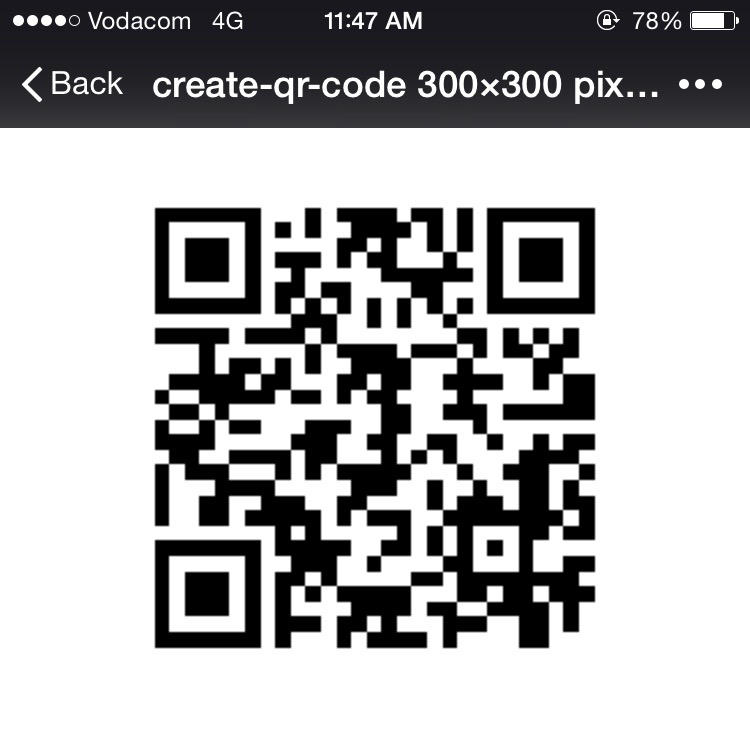
\includegraphics[width=0.5\textwidth]{figs/qr_code.jpg}
   \caption{Generated QR-code} 
   \label{fig:qr_code}
\end{figure}

\subsubsection{QR-code to Address}
Our second design spesifiction is to allow a user to scan a QR-code to make a payment to. Although the WeChat application has a QR-code reader built-in, it doesn't allow the user to scan a QR-code directly from an Official Account. An Official Account does allow a user to send an image to our server. This will allow us to decode the QR-code on our server. For simplicity, we decided to use a third-party service called goQR.me to decode the QR-code. WeChat sends our server a link of the image that the user sent. This link of the image is used by the third-party service and responds with the decoded text. The bitcoin-lib-php software can verify that the decoded text is a valid Bitcoin address.

This method of decoding the QR-code is very computationally- and bandwidth efficient for our server, since the image itself is not sent through our server. Just like the Bitcoin Interface in section \ref{sct:bitcoin_interface_design}, we chose to use a third-party service for our proof of concept. If we were to build the service for production scale, we would rather exchange the third-party service for our own software. In the case of the QR-code service, it would be a major security concern to use a third-party service. A malicious third-party can exchange the correct address with their own address to receive Bitcoin that is not intended for them.



\subsubsection{User Balance}

Getting the balance of the user's address is the second core feature that a Bitcoin wallet application requires. Calculating an address' balance involves summing all the user's unspent outputs. Fortunately, the Chain.com API allows us to retrieve the balance of any Bitcoin address directly using a single method call. The result of getting the balance can be seen in figure \ref{fig:wechat_balance}.

\begin{figure}
  \centering
    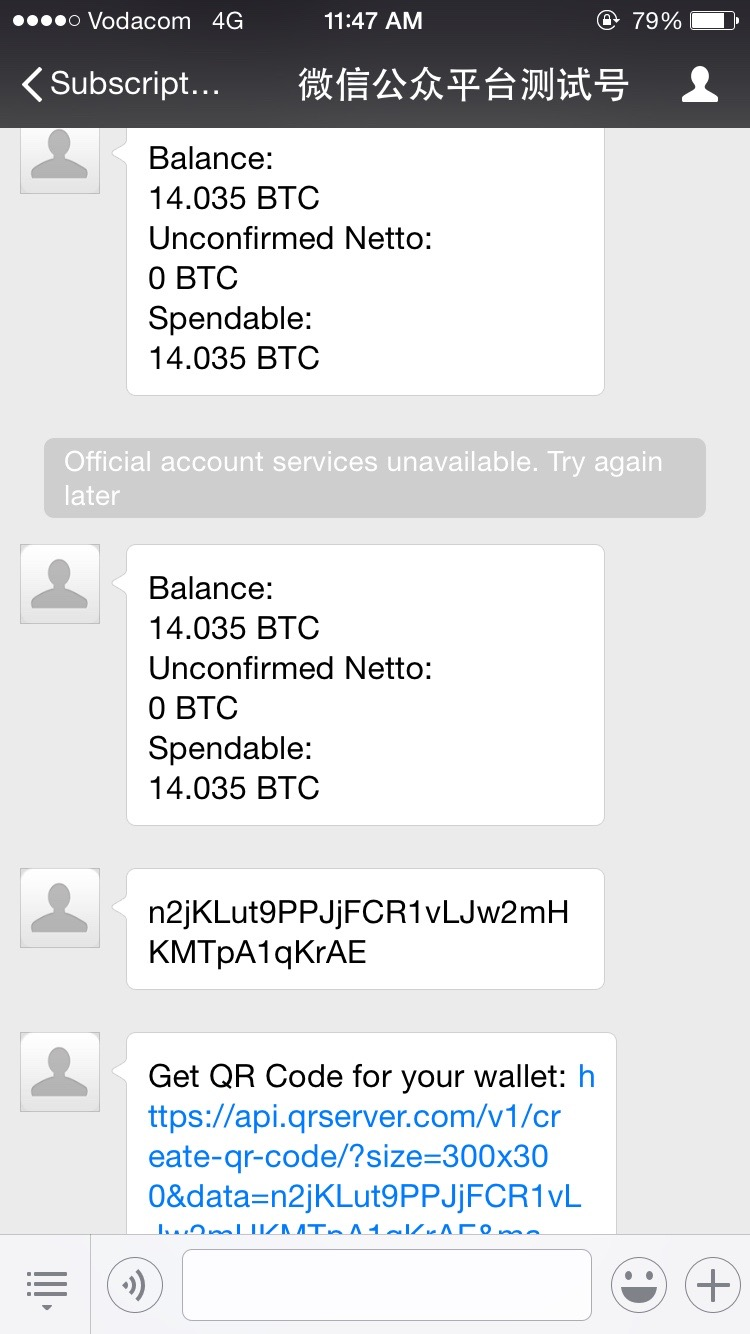
\includegraphics[width=0.3\textwidth]{figs/wechat_balance.jpg}
   \caption{WeChat Balance} 
   \label{fig:wechat_balance}
\end{figure}

\subsubsection{Make A Payment}

The core process of making a payment is handled in section \ref{sct:bitcoin_interface_design} and can be seen in figure \ref{fig:bitcoin_payment_flow}. The most important part of the payment flow is that the user's Bitcoin private key never leaves our server, even though a third-party service is used to publish the transaction. 


\section{REST API Design}

There are many ways to implement a REST API. This is because of the ``black-box'' approach of REST. As such, the first major design decision that needs to be made is whether to use a REST framework or two build it from scratch. Using a REST framework would be easier and standardized and if the framework is maintained it would also be secure.

In spite of the advantages of using a REST framework, we decided to build it ourself. The motivation for choosing this method is that the author wanted to get a better understanding of how a REST API works on the low-level and felt that building it from scratch would give a better understanding. Thus, we will use the same tools to build the other parts of our system, ie. PHP and MySQL.

\subsection{REST Endpoints}

A PHP script is usually called in the following format: ``url/script.php''. However, for a REST API we need a clean URL in the format: ``url/script''. Since we are using an Apache server, we need to modify the ``.htaccess'' file with regular expressions.

Thus, we have different regular expressions in the .htaccess file that will call a single script with the corresponding parameters from the request. The .htaccess file will only relay the parameters of the url to the PHP script. The PHP script will then apply logic to determine what function should be executed. 

The PHP script will firstly authenticate the developer, followed by the do the corresponding external API calls, database entries, response HTTP status code and JSON response data.

\begin{figure}
  \centering
    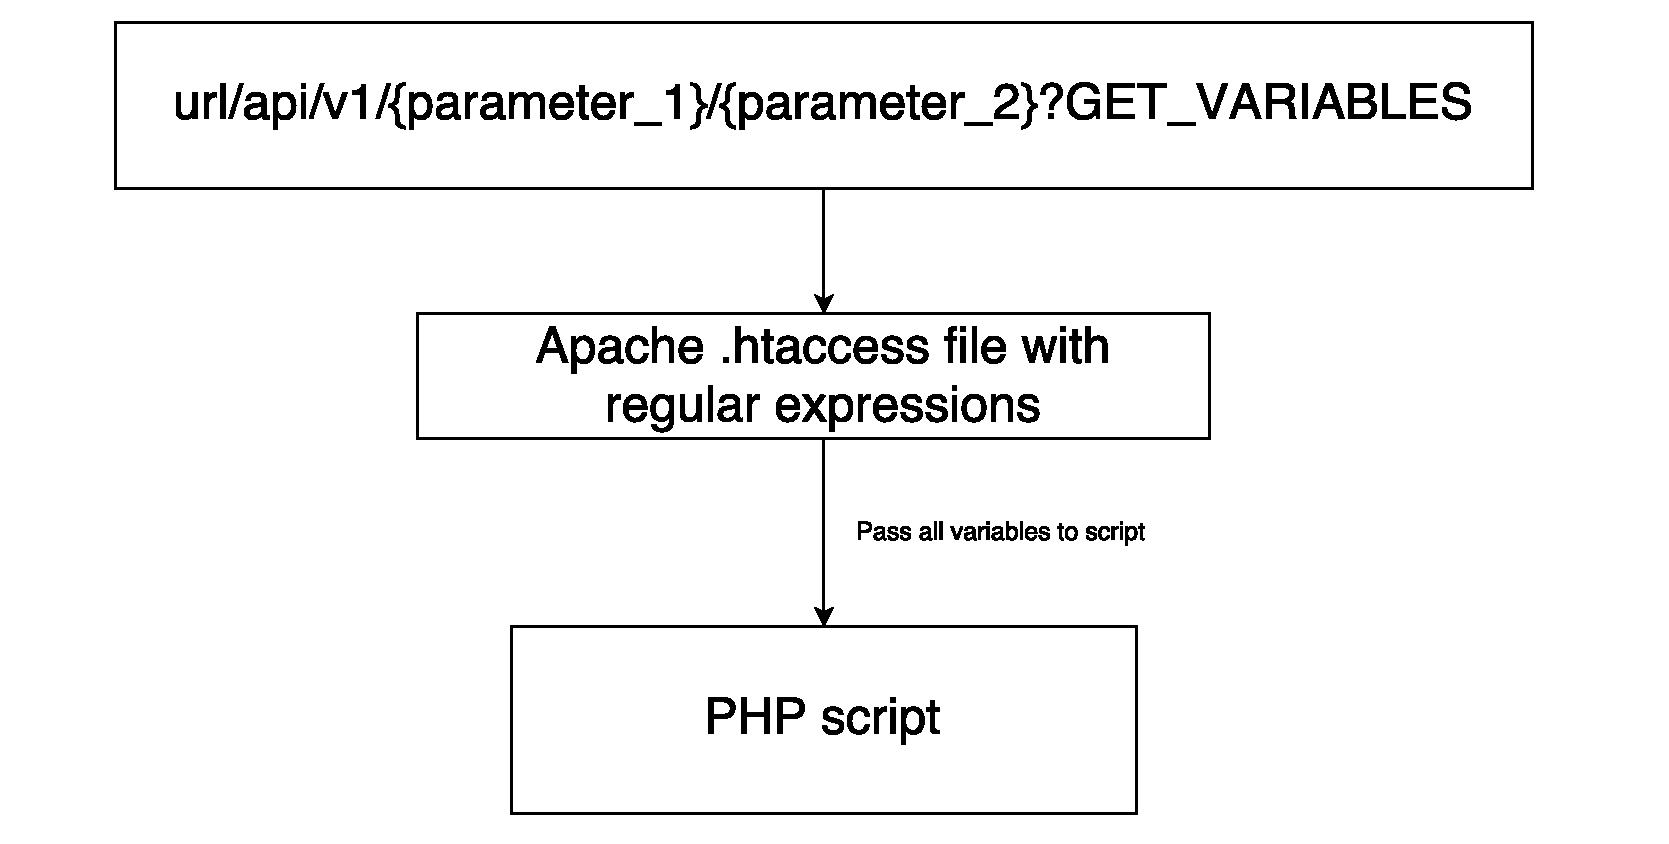
\includegraphics[width=0.8\textwidth]{figs/htaccess_file.pdf}
   \caption{REST URL Flow} 
   \label{fig:htaccess_file}
\end{figure}

The following is an excerpt from the .htaccess file that is responsible for the routing of the REST endpoints:
\begin{tiny}
\begin{verbatim}
RewriteRule ^api/v1/([A-Za-z0-9-]+)/([A-Za-z0-9-]+)/?$ 
/chaintest/my_api.php?first_query=$1&second_query=$2 [NC,QSA,L]

RewriteRule ^api/v1/([A-Za-z0-9-]+)/?$ /chaintest/my_api.php?first_query=$1 [NC,QSA,L]

RewriteRule ^api/v1/?$ /chaintest/my_api.php
\end{verbatim}
\end{tiny}

The first RewriteRule matches queries with two parameters in the URI and turns the parameters into GET variables first\_query and second\_query. The my\_api.php script will then be able to access these variables like normal GET variables. 

\begin{table}
	\begin{center}
		\begin{tabular}	{ | c | p{7cm} |}
		\hline
		Flag & Description \\ \hline
		NC & No Case. Doesn't differentiate between upper- and lower case. \\ \hline
		QSA & Query String Append. Adds the variables to the existing GET variables. \\ \hline
		L & Last. If the rule matches, no further rules will be processed. \\ \hline
		
		
	   % \label{fig:htaccess_file}
		\end{tabular}
		\caption{Table of selected .htaccess flags} 
		\label{tbl:htaccess_flags}
	\end{center}
\end{table}
